\documentclass[10pt,a4paper]{article}
\usepackage[margin=2.1cm,top=2.4cm,bottom=2.2cm]{geometry}
\usepackage{amsmath,amssymb,mathtools,graphicx,booktabs,xspace,fancyhdr,array,microtype}
\usepackage[hidelinks]{hyperref}
\graphicspath{{results/}}
% generated by code/main.py -- do not edit
\newcommand{\ParamGroup}{S\xspace}
\newcommand{\ParamN}{200\xspace}
\newcommand{\ParamM}{1200\xspace}
\newcommand{\ParamSigma}{\ensuremath{1\times10^{-3}}\xspace}
\newcommand{\ParamSeed}{0\xspace}
\newcommand{\ParamGradTol}{\ensuremath{1\times10^{-8}}\xspace}
\newcommand{\ParamDeltaZero}{1.0\xspace}
\newcommand{\ParamDeltaBar}{100\xspace}
\newcommand{\ParamRhoPrime}{0.1\xspace}
\newcommand{\ParamKappa}{0.1\xspace}
\newcommand{\ParamTheta}{1\xspace}
\newcommand{\ParamNStarts}{10\xspace}
\newcommand{\NumTestsTotal}{19\xspace}
\newcommand{\NumTestsPassed}{19\xspace}
\newcommand{\CheckSlopeGrad}{2.00\xspace}
\newcommand{\CheckSlopeHess}{3.00\xspace}
\newcommand{\TimeHessVecFree}{\ensuremath{1.7\times10^{-4}}\xspace}
\newcommand{\TimeHessDenseBuild}{\ensuremath{2.8\times10^{-3}}\xspace}
\newcommand{\TimeHessDenseMatVec}{\ensuremath{8.0\times10^{-6}}\xspace}
\newcommand{\TimeHessRatio}{16\xspace}
\newcommand{\HessDiffNorm}{\ensuremath{5.1\times10^{-16}}\xspace}
\newcommand{\TRIters}{17\xspace}
\newcommand{\TRMatvecs}{218\xspace}
\newcommand{\TRTime}{\ensuremath{1.93\times10^{-2}}\xspace}
\newcommand{\TRFinalGrad}{\ensuremath{8.0\times10^{-14}}\xspace}
\newcommand{\TRFinalErr}{\ensuremath{2.35\times10^{-3}}\xspace}
\newcommand{\TRFinalCost}{\ensuremath{5.46\times10^{-7}}\xspace}
\newcommand{\TRSign}{-\xspace}
\newcommand{\TRRejected}{0\xspace}
\newcommand{\TRTotalTCG}{91\xspace}
\newcommand{\TRMaxTCG}{31\xspace}
\newcommand{\TRNegCurv}{1\xspace}
\newcommand{\TRBoundary}{5\xspace}
\newcommand{\TRTolerance}{11\xspace}
\newcommand{\TRDeltaMax}{8.0\xspace}
\newcommand{\TRIterGradBelowEThree}{15\xspace}
\newcommand{\GDIters}{13839\xspace}
\newcommand{\GDMatvecs}{41517\xspace}
\newcommand{\GDTime}{\ensuremath{3.16\times10^{0}}\xspace}
\newcommand{\GDFinalErr}{\ensuremath{2.35\times10^{-3}}\xspace}
\newcommand{\GDGradAtTRBudget}{\ensuremath{8.2\times10^{-3}}\xspace}
\newcommand{\GDErrAtTRBudget}{\ensuremath{1.2\times10^{0}}\xspace}
\newcommand{\SpeedupMatvecs}{190\xspace}
\newcommand{\SpeedupTime}{164\xspace}
\newcommand{\SpeedupIters}{814\xspace}
\newcommand{\CostAtTrue}{\ensuremath{8.43\times10^{-7}}\xspace}
\newcommand{\InitialErr}{1.36\xspace}
\newcommand{\InitialGrad}{\ensuremath{3.7\times10^{0}}\xspace}
\newcommand{\NormXTrue}{13.9\xspace}
\newcommand{\MSTRSuccess}{10\xspace}
\newcommand{\MSGDSuccess}{10\xspace}
\newcommand{\MSTRItersMin}{14\xspace}
\newcommand{\MSTRItersMax}{40\xspace}
\newcommand{\MSTRMatvecsMedian}{223\xspace}
\newcommand{\MSGDMatvecsMedian}{42460\xspace}
\newcommand{\MSTRTimeMedian}{\ensuremath{1.65\times10^{-2}}\xspace}
\newcommand{\MSGDTimeMedian}{\ensuremath{3.16\times10^{0}}\xspace}
\newcommand{\MSErrMax}{\ensuremath{2.35\times10^{-3}}\xspace}
\newcommand{\EigAtAMax}{300\xspace}
\newcommand{\EigAtAMin}{0.18\xspace}
\newcommand{\EigAtAMedian}{0.47\xspace}
\newcommand{\CondAtA}{1683\xspace}
\newcommand{\EigHessMin}{\ensuremath{1.42\times10^{-4}}\xspace}
\newcommand{\EigHessMax}{0.4\xspace}
\newcommand{\CondHess}{2930\xspace}
   % all numbers below are generated by code/main.py

% ---- TODO(group): put the real member names here --------------------------------
\newcommand{\groupmembers}{Name 1, Name 2, Name 3, Name 4}
% ------------------------------------------------------------------------------------
\newcommand{\inner}[2]{\langle #1,#2\rangle}
\newcommand{\R}{\mathbb{R}}
\newcommand{\D}{\mathrm{D}}
\newcommand{\xtrue}{x_{\mathrm{true}}}
\newcommand{\code}[1]{\texttt{#1}}
\pagestyle{fancy}\fancyhf{}
\fancyhead[L]{MATH-329 -- Homework 2}\fancyhead[R]{Group \ParamGroup}
\fancyfoot[L]{\footnotesize Group \ParamGroup: \groupmembers}\fancyfoot[R]{\thepage}
\setlength{\parindent}{0pt}\setlength{\parskip}{4pt}

\begin{document}
\begin{center}
{\Large\bfseries Homework 2: trust-region methods for real phase retrieval}\\[2pt]
Group \ParamGroup\ --- \groupmembers
\end{center}

\textbf{Reproducibility.} \code{python code/main.py} (run from \code{code/}) executes the tests, the derivative
checks and all experiments, writes every figure and table to \code{results/} and every number quoted below to
\code{results/numbers.tex}, which this file \verb|\input|s: report, code and results come from one run.
Instance: $n=\ParamN$, $m=\ParamM$, $\sigma=\ParamSigma$, seed \ParamSeed\ (\code{generate\_data}, same draw order as the handout).
Code names used below: \code{tcg} (\code{tcg.py}), \code{trust\_region\_tcg} (\code{trust\_region.py}),
\code{cost}, \code{grad}, \code{hess\_vec} (\code{phase\_retrieval.py}), \code{gradient\_descent}, \code{tests.py}.

\section*{Question 1 -- truncated CG}
\code{tcg(Hv, g, Delta)} solves $\min_{\|v\|\le\Delta} m(v)=\tfrac12\inner{v}{Hv}+\inner gv$ with Steihaug--Toint CG started at $v_0=0$,
$r_0=g$, $p_0=-g$; \code{Hv} is a \emph{function} $v\mapsto Hv$, so $H$ is never formed. At each iteration, if
$\inner{p}{Hp}\le0$ or the CG step leaves the ball, we move along $p$ to the boundary, i.e.\ to the positive root $\tau$ of
$\|v+\tau p\|=\Delta$ (computed in the cancellation-free form $\tau=-2c/(b+\sqrt{b^2-4ac})$ when $b\ge0$). Otherwise we stop when
$\|r\|\le\|g\|\min(\kappa,\|g\|^{\theta})$ with $\kappa=\ParamKappa$, $\theta=\ParamTheta$, or after $n$ iterations. The function also returns
$Hv$ (tracked recursively, free of extra products) and $m(0)-m(v)$, which TR-tCG needs. Corner case: for $g=0$ it returns $v=0$ (even if $H$ has
negative curvature, as for any CG-based solver).

\textbf{Tests} (all in \code{tests.py}; \NumTestsPassed\ of \NumTestsTotal\ pass in the final run; list below, 1-D/2-D/3-D cases have known solutions):
{\scriptsize
\begin{center}
\begin{tabular}{@{}p{5.6cm}p{9.6cm}c@{}}
\toprule function & what is checked & result\\\midrule
\texttt{test\_tcg\_1d\_interior} & tCG 1-D, minimiser strictly inside the ball & pass \\
\texttt{test\_tcg\_1d\_boundary} & tCG 1-D, minimiser outside: stops on the boundary & pass \\
\texttt{test\_tcg\_1d\_negative\_curvature} & tCG 1-D, concave model: goes to the correct boundary point & pass \\
\texttt{test\_tcg\_zero\_gradient} & tCG corner case $g=0$ returns $v=0$ & pass \\
\texttt{test\_tcg\_zero\_hessian} & tCG with $H=0$: boundary step along $-g$ & pass \\
\texttt{test\_tcg\_tiny\_radius} & tCG with tiny $\Delta$: Cauchy-like step $-\Delta g/\|g\|$ & pass \\
\texttt{test\_tcg\_2d\_negative\_curvature} & tCG 2-D indefinite $H$, exact solution known & pass \\
\texttt{test\_tcg\_3d\_interior\_equals\_newton} & tCG 3-D, large ball, tiny tolerance: equals $-H^{-1}g$ & pass \\
\texttt{test\_tcg\_singular\_psd\_in\_range} & tCG 3-D singular PSD $H$, $g\in\mathrm{range}(H)$ & pass \\
\texttt{test\_tcg\_singular\_psd\_outside\_range} & tCG 2-D singular PSD $H$, zero curvature along $-g$ & pass \\
\texttt{test\_tcg\_random\_properties} & 200 random indefinite models: feasibility, Cauchy decrease, tracked $Hv$ & pass \\
\texttt{test\_tcg\_matrix\_free\_callable} & tCG only needs a function $v\mapsto Hv$ & pass \\
\texttt{test\_tr\_quadratic} & TR-tCG on a strongly convex quadratic finds $Q^{-1}b$ & pass \\
\texttt{test\_tr\_rosenbrock} & TR-tCG on Rosenbrock reaches $(1,1)$, $f$ monotone & pass \\
\texttt{test\_tr\_escapes\_saddle} & TR-tCG leaves a saddle point (negative curvature) & pass \\
\texttt{test\_tr\_radius\_rules} & TR-tCG radius updates respect $\bar\Delta$ and doubling rule & pass \\
\texttt{test\_grad\_vs\_dense\_formula} & gradient equals explicit formula & pass \\
\texttt{test\_hessvec\_vs\_dense\_and\_symmetry} & Hessian-vector product equals dense Hessian; symmetry & pass \\
\texttt{test\_hessvec\_vs\_finite\_difference\_of\_gradient} & Hessian-vector product vs central differences of $\nabla f$ & pass \\
\bottomrule

\end{tabular}
\end{center}}

\section*{Question 2 -- TR-tCG}
\code{trust\_region\_tcg(problem, x0, \dots)} needs only \code{cost}, \code{grad} and \code{hess\_op(x)} (returning $v\mapsto\nabla^2 f(x)[v]$).
At $x_k$ it calls \code{tcg} on $m_k(s)=f(x_k)+\inner{\nabla f(x_k)}s+\frac12\inner{s}{\nabla^2f(x_k)s}$ with radius $\Delta_k$, sets
$\rho_k=\frac{f(x_k)-f(x_k+s_k)}{m_k(0)-m_k(s_k)}$ (numerator and denominator are shifted by $10^3\varepsilon_{\mathrm{mach}}\max(1,|f|)$ against round-off near convergence),
accepts the step iff $\rho_k>\rho'=\ParamRhoPrime$, and updates $\Delta$: $\Delta/4$ if $\rho<\frac14$; $\min(2\Delta,\bar\Delta)$ if $\rho>\frac34$ and
$\|s_k\|=\Delta_k$; unchanged otherwise. Parameters: $\Delta_0=\ParamDeltaZero$, $\bar\Delta=\ParamDeltaBar$; stop when $\|\nabla f\|\le\ParamGradTol$.
Gradient and Hessian operator are recomputed only after an accepted step. Tests (the four \code{test\_tr\_*} rows of the table): a strongly convex quadratic
(solution $Q^{-1}b$ in few iterations), Rosenbrock (where $\nabla f,\nabla^2f$ are known; $f$ decreases monotonically), a saddle that the method must leave
via negative curvature, and the radius rules on $f(x)=\|x\|^2$.

\section*{Question 3 -- derivatives of $f(x)=\frac1{4n}\|(Ax)^{\odot2}-y^{\odot2}\|^2$}
Let $z=Ax$ and $r=z^{\odot2}-y^{\odot2}$, so $f=\frac1{4n}\|r\|^2$. Then $\D z[v]=Av$ and $\D r[v]=2\,z\odot Av$, hence
\[
\D f(x)[v]=\tfrac1{2n}\inner{r}{\D r[v]}=\tfrac1n\inner{r}{z\odot Av}=\tfrac1n\inner{r\odot z}{Av}=\inner{\tfrac1nA^{\top}(r\odot z)}{v},
\]
using $\inner{u\odot v}{w}=\inner{u}{w\odot v}$ in the third equality. Therefore
\[
\boxed{\nabla f(x)=\tfrac1n A^{\top}\!\big(z^{\odot3}-y^{\odot2}\odot z\big)}\,.
\]
Differentiating again, with $\D z[v]=Av$ and $\D r[v]=2z\odot Av$:
\[
\boxed{\nabla^2 f(x)[v]=\tfrac1n A^{\top}\!\big((2z^{\odot2}+r)\odot Av\big)=\tfrac1n A^{\top}\!\big((3z^{\odot2}-y^{\odot2})\odot Av\big)}\,,
\]
which costs two products with $A$/$A^\top$ ($O(mn)$) instead of forming the $n\times n$ Hessian $\frac1nA^\top\mathrm{diag}(3z^{\odot2}-y^{\odot2})A$ ($O(mn^2)$).
The Hessian-vector product agrees with the dense Hessian to relative error \HessDiffNorm; on this machine (one core) one product costs
\TimeHessVecFree\ s, whereas building the dense Hessian costs \TimeHessDenseBuild\ s ($\approx\TimeHessRatio\times$ more at $n=\ParamN$; the gap grows linearly with $n$).

\textbf{Numerical checks} (\code{main.py}, figure below): at $x=x_0$ and a random unit $v$, $|f(x+tv)-f(x)-t\inner{\nabla f(x)}v|=O(t^2)$ and
$|f(x+tv)-f(x)-t\inner{\nabla f(x)}v-\frac{t^2}2\inner{v}{\nabla^2f(x)[v]}|=O(t^3)$. The fitted log-log slopes are \CheckSlopeGrad\ and \CheckSlopeHess\ (expected 2 and 3),
on windows $t\in[10^{-4},10^{-2}]$ and $[10^{-3},3\cdot10^{-2}]$; for smaller $t$ the curves flatten and fluctuate at the round-off level ($\approx\varepsilon_{\mathrm{mach}}|f|$), and for larger $t$ the higher-order terms of the quartic take over. Additional tests: symmetry $\inner u{Hv}=\inner v{Hu}$ and central differences of $\nabla f$.
\begin{center}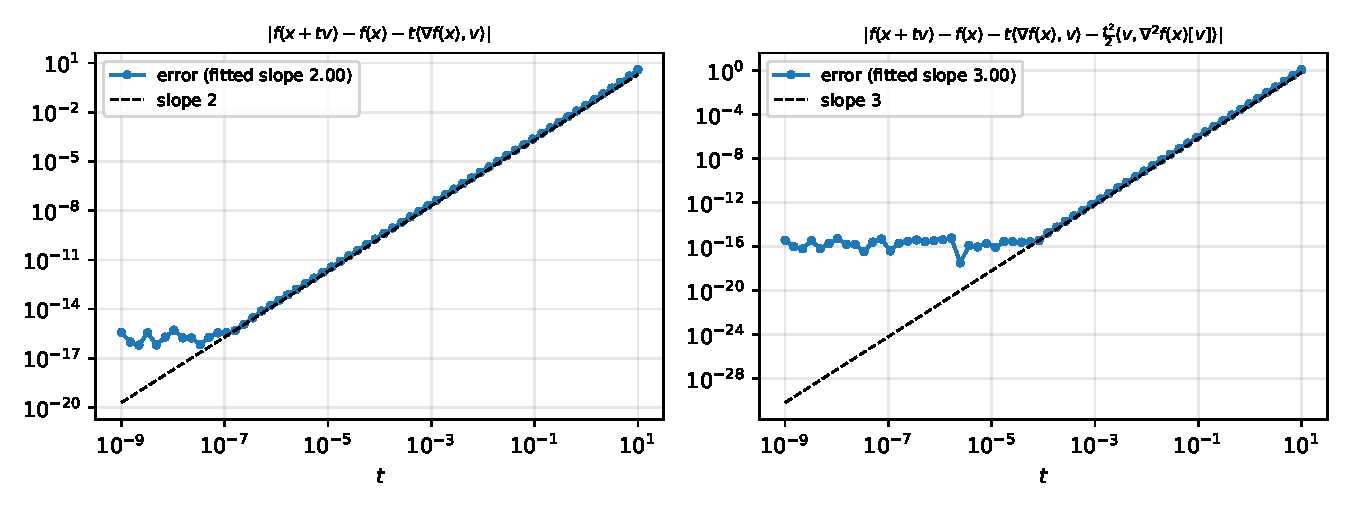
\includegraphics[width=0.86\textwidth]{fig_derivative_checks.pdf}\end{center}

\section*{Question 4 -- running TR-tCG}
Starting from $x_0$ (initial error $e(x_0)=\InitialErr$, $\|\nabla f(x_0)\|=\InitialGrad$), TR-tCG reaches $\|\nabla f\|\le\ParamGradTol$ in \TRIters\ iterations
(\TRMatvecs\ products with $A$ or $A^\top$, \TRTime\ s) with $e(x)=\TRFinalErr$; it converges to $\TRSign\xtrue$ (the sign ambiguity), and the final
gradient norm is \TRFinalGrad. \TRRejected\ steps were rejected; $\Delta$ grew up to \TRDeltaMax; tCG stopped on tolerance \TRTolerance\ times, on the boundary \TRBoundary\ times,
on negative curvature \TRNegCurv\ time(s), with at most \TRMaxTCG\ tCG iterations per call. The gradient norm drops below $10^{-3}$ at iteration \TRIterGradBelowEThree\
and then collapses (super-linear/quadratic phase). The error plateaus at $\approx\TRFinalErr$: this is the noise floor ($\sigma=\ParamSigma$, and the minimiser of $f$ is not $\xtrue$:
$f(\xtrue)=\CostAtTrue>\TRFinalCost=f(x_{\mathrm{end}})$), not an algorithmic failure.
\begin{center}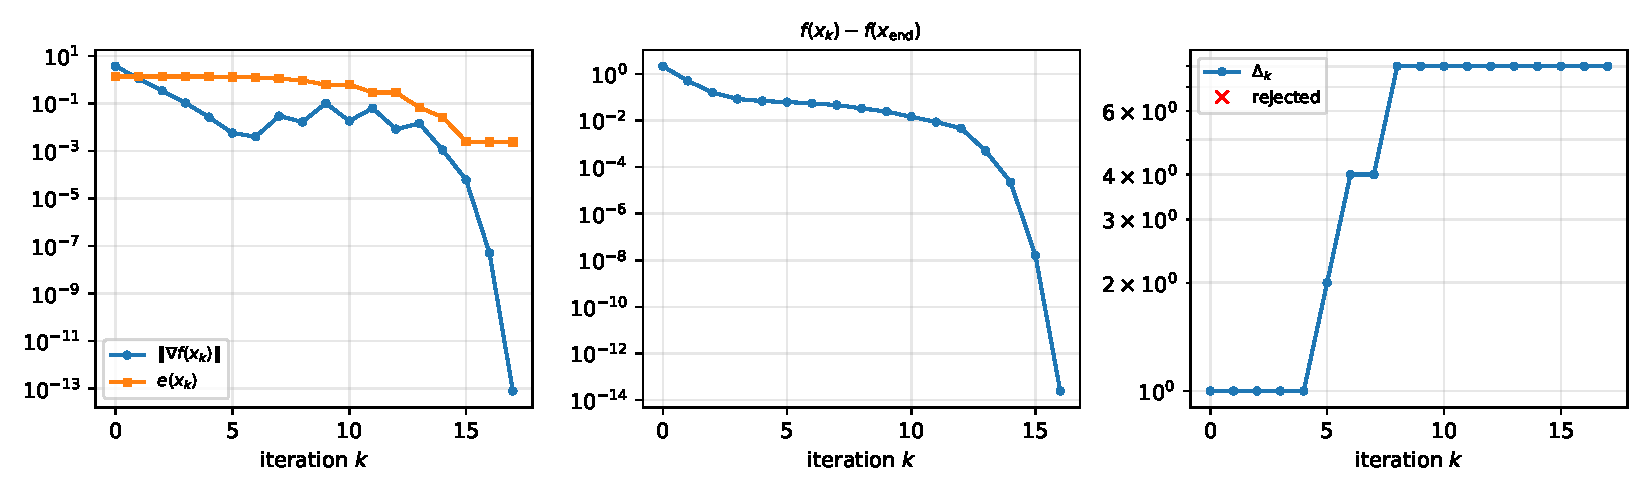
\includegraphics[width=\textwidth]{fig_trtcg.pdf}\end{center}

\textbf{Comparison with gradient descent} (\code{gradient\_descent}: Armijo backtracking, $c_1=10^{-4}$, halving, first trial $=2\times$ previous accepted step), same $x_0$,
same stopping rule. 
\begin{center}\small
\begin{tabular}{lrrrr}\toprule & iterations & products with $A,A^\top$ & time (s) & final $e(x)$\\\midrule
TR-tCG & \TRIters & \TRMatvecs & \TRTime & \TRFinalErr\\
GD + Armijo & \GDIters & \GDMatvecs & \GDTime & \GDFinalErr\\\bottomrule\end{tabular}
\end{center}
TR-tCG needs about \SpeedupMatvecs$\times$ fewer products and is about \SpeedupTime$\times$ faster in wall-clock time (\SpeedupIters$\times$ fewer iterations, but iterations are not comparable).
With the \emph{same budget} of \TRMatvecs\ products GD only reaches $\|\nabla f\|=\GDGradAtTRBudget$ and $e=\GDErrAtTRBudget$.
\begin{center}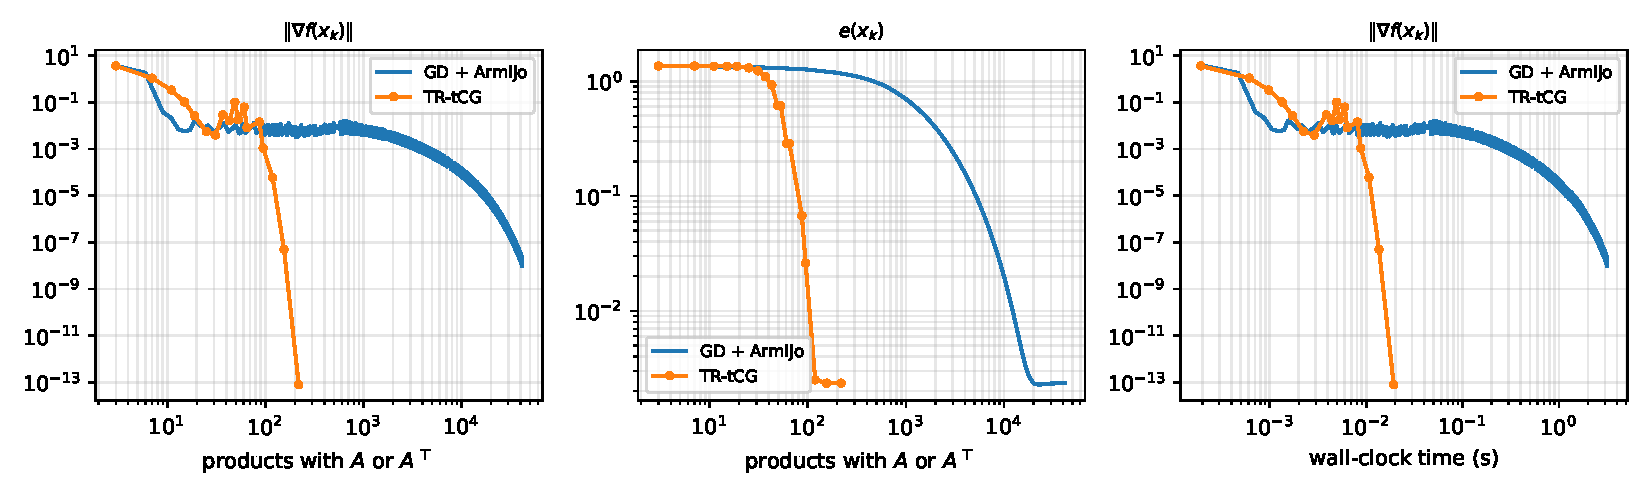
\includegraphics[width=\textwidth]{fig_comparison.pdf}\end{center}

\textbf{Robustness.} Over \ParamNStarts\ further random starting points (same $A,y$; same $x_0$ for both methods), TR-tCG recovered $\pm\xtrue$ (error $<10^{-2}$) in \MSTRSuccess/\ParamNStarts\ runs
(\MSTRItersMin--\MSTRItersMax\ iterations; median \MSTRMatvecsMedian\ products, \MSTRTimeMedian\ s; worst error \MSErrMax) and GD in \MSGDSuccess/\ParamNStarts\ runs
(median \MSGDMatvecsMedian\ products, \MSGDTimeMedian\ s).

\textbf{What should one pay attention to for a fair comparison?}
(i) Same instance, same $x_0$, same stopping criterion $\|\nabla f\|\le\ParamGradTol$, and neither method sees $\xtrue$ (the error is computed afterwards from stored iterates and excluded from the timers).
(ii) Count work in a common unit, not iterations: a TR iteration contains several tCG Hessian-vector products (about \TRTotalTCG\ in total), plus the cost of rejected steps, whereas a GD iteration contains
line-search function evaluations; we count \emph{every} product with $A$ or $A^\top$ and also report wall-clock time (both implementations are vectorised, reuse $Ax$ when possible, and use the same counters).
(iii) Compare at equal accuracy and in the sign-invariant error $e(x)$, not $\|x-\xtrue\|$.
(iv) GD is not a straw man (adaptive initial step with Armijo) but is still the simplest first-order method; momentum, Barzilai--Borwein steps or L-BFGS would shrink the gap, and the TR parameters
($\Delta_0,\bar\Delta,\kappa,\theta$) were not tuned either. (v) One instance and one run is anecdotal and timings are noisy: hence the multi-start medians above.

\section*{Question 5 -- what did we learn?}
% TODO(group): rewrite in your own words, based on your own experience (the course asks for genuine reflections).
\emph{Draft based on what the final run shows.}
(1) The sign ambiguity is real: TR-tCG converged to $\TRSign\xtrue$, so judging by $\|x-\xtrue\|$ would have suggested failure; $e(x)$ is the right metric.
(2) Conditioning explains the gap with GD: the entries of $A$ have mean $\frac1{2\sqrt n}\ne0$, so $A^\top A$ has one huge eigenvalue (\EigAtAMax) and a bulk around \EigAtAMedian\
(condition number \CondAtA). At the computed solution the Hessian is positive definite, with $\lambda_{\min}=\EigHessMin$, $\lambda_{\max}=\EigHessMax$ (condition number \CondHess), so GD with a safe step
needs thousands of iterations, while TR-tCG uses curvature information and ends with quadratic-like convergence.
(3) Matrix-free Hessian-vector products are what make TR-tCG cheap: the identity $\inner{u\odot v}w=\inner u{w\odot v}$ turns the derivatives into two products with $A,A^\top$ each, and the
dense Hessian is about \TimeHessRatio$\times$ more expensive to build at $n=\ParamN$. In the Taylor tests, round-off dominates for very small $t$, so slopes must be read on a suitable window of $t$.
(4) Details that matter in the implementation: the cancellation-free formula for the boundary step $\tau$, the regularisation of $\rho$ near convergence, and the corner case $g=0$ in tCG; tests with known answers
(1-D/2-D/3-D) check each of them separately. (5) All \ParamNStarts\ random starts converged to $\pm\xtrue$ despite non-convexity, and tCG needed at most \TRMaxTCG\ iterations per TR step, far fewer than $n=\ParamN$.
% TODO(group): add your own difficulties, realizations and surprises.

\end{document}
